\section{Ontology}

\begin{requirement}
    \label{requirement:ontologies-on-the-web}
    As many ontologies are located on the web in formats such as OWL (Web Ontology Language), RDFs (RDF Schema), UFO (Unified Foundational Ontology), etc., the application shall support reading them.
\end{requirement}

It may seem that designing the ontology directly in the tool is beneficial because a user does not need to use other tools and the application may already build the schema, which is a feedback to the user. This approach was used in tools \textit{XCase} and \textit{eXolutio} as can be seen in the \autoref{fig:exolutio} in the left panel. However, it has the following drawbacks:

\begin{enumerate}
    \item Designing an ontology is a well-defined problem. There are many great and time-proven tools we could not cope with.
    \item Even if the ontology will be used just to generate the schemas, it may be worthy of publishing it anyways as others may benefit from it.
    \item It is better to split a complex problem into smaller ones.
\end{enumerate}

On the other hand, not having direct access to the ontology, as it will be on the Web, has the following impacts:

\begin{enumerate}
    \item The ontology may \textbf{not always be available}. Unavailability should not prevent us from generating the schemas and making minor changes to them if those changes are not directly related to exploring the ontology.
    \item The concepts in the ontology may \textbf{point to another ontology} according to the Linked Data principles.
\end{enumerate}

For the reasons mentioned above, the preferred workflow is to design the ontology separately in the external tool, publish it on the Web, and then model the schema in the application. There is \autoref{requirement:pim-editing} later in the text specifying that a user can make modifications in the application. This is not inconsistent with the statements, as it deals with minor changes instead of defining a complete ontology.

The term ontology has already been defined in the introductory chapter, and we will formally define its specific requirements in the next chapter.

It shall be easy to implement support for other types of ontologies, and all of them shall be linkable according to the LD principles.

\subsection{Format of the ontology}

In the above requirement, several different formats were proposed for the ontology. This section will analyze the minimal requirements for any ontology format and how we will treat additional information in them. Because the core goal is to design schemas, we will start with a model proposed from \autoref{requirement:general-schema}. The schema consists of classes and their properties. A class corresponds to a thing from real life. An attribute is a literal that belongs to the given class only. On the other hand, an association is a link between two (not necessarily different) classes. From this point of view, the association is an independent entity.

Associations are usually oriented, and some ontologies may specify a title and a description for a reverse direction. For example, in RDFS, the association (or property in the RDFS terminology) is an entity of type {\tt rdf:Property} having domain and range classes and a title and description. Therefore, it only describes the forward direction. We can, of course, create a property in the other direction as well, but there would not be a connection between a forward and a reverse direction. Hence, we would not know that those are semantically the same properties. UFO (Unified Foundational Ontology), as an example of a more complex ontology, introduces relators. Relators are relationships between two or more things connected by mediation. The mediation can be described, giving us a way to describe both directions differently.

Although the latter approach is more complex, using simple concepts for associations may be disadvantageous for the aforementioned reason. Therefore, we will follow the pattern of UFO and any other simpler ontologies, such as RDFS, will not have the reverse direction described.

\medskip

An ontology in the context of this requirement is a set of classes that have attributes. The associations then connect two classes together. The connected classes may not have the same ontology.

As some formats specify the ontology in a more complex way, the application may use the additional information to better design the schema. This statement is better defined in the next chapter.

\begin{figure}[h!]\centering
  \centering
  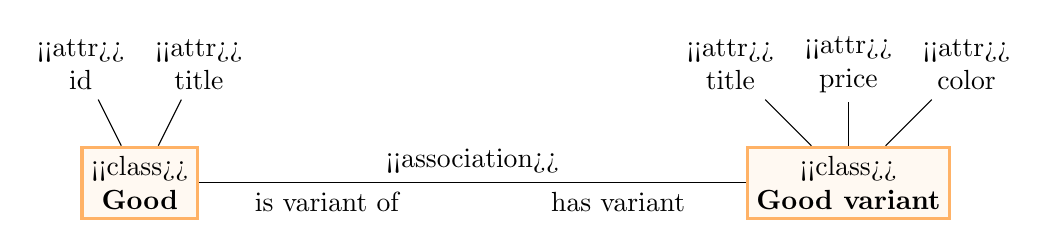
\begin{tikzpicture}[
    class/.style={shape=rectangle, draw=orange!60, fill=orange!5, very thick, minimum size=5mm,align=center},
    attribute/.style={align=center},
  ]
    \node[class] (good) at (0,0) {<<class>>\\\textbf{Good}};
    \node[class] (variant) at (9,0) {<<class>>\\\textbf{Good variant}};

    \node[attribute] (a11) at (-.75,1.5) {<<attr>>\\id};
    \node[attribute] (a12) at (.75,1.5) {<<attr>>\\title};

    \node[attribute] (a21) at (7.5,1.5) {<<attr>>\\title};
    \node[attribute] (a22) at (9,1.5) {<<attr>>\\price};
    \node[attribute] (a23) at (10.5,1.5) {<<attr>>\\color};

    \draw (good) -- (a11);
    \draw (good) -- (a12);

    \draw (variant) -- (a21);
    \draw (variant) -- (a22);
    \draw (variant) -- (a23);

    \draw (good) -- node[pos=0.225,below]{$\blacktriangleleft$ is variant of} node[above]{<<association>>} node[pos=0.775,below]{has variant $\blacktriangleright$} (variant);
  \end{tikzpicture}

  \caption{Schematic diagram of an ontology which could be used for the schema from the \autoref{analysis/general-schema-representation}.}
\end{figure}

% todo popis, jak by mela ontologie vypadat na zaklade toho schematu. Jakou by mela mit strukturu a co musi obsahovat

% mozna ze to je jak uml